\section{Conclusion}
\begin{frame}{Summary}
\begin{columns}
\begin{column}{0.4\textwidth}
	\begin{overlayarea}{\textwidth}{\textheight}
		\centering
		\only<1>{\vspace{-0.08\textheight}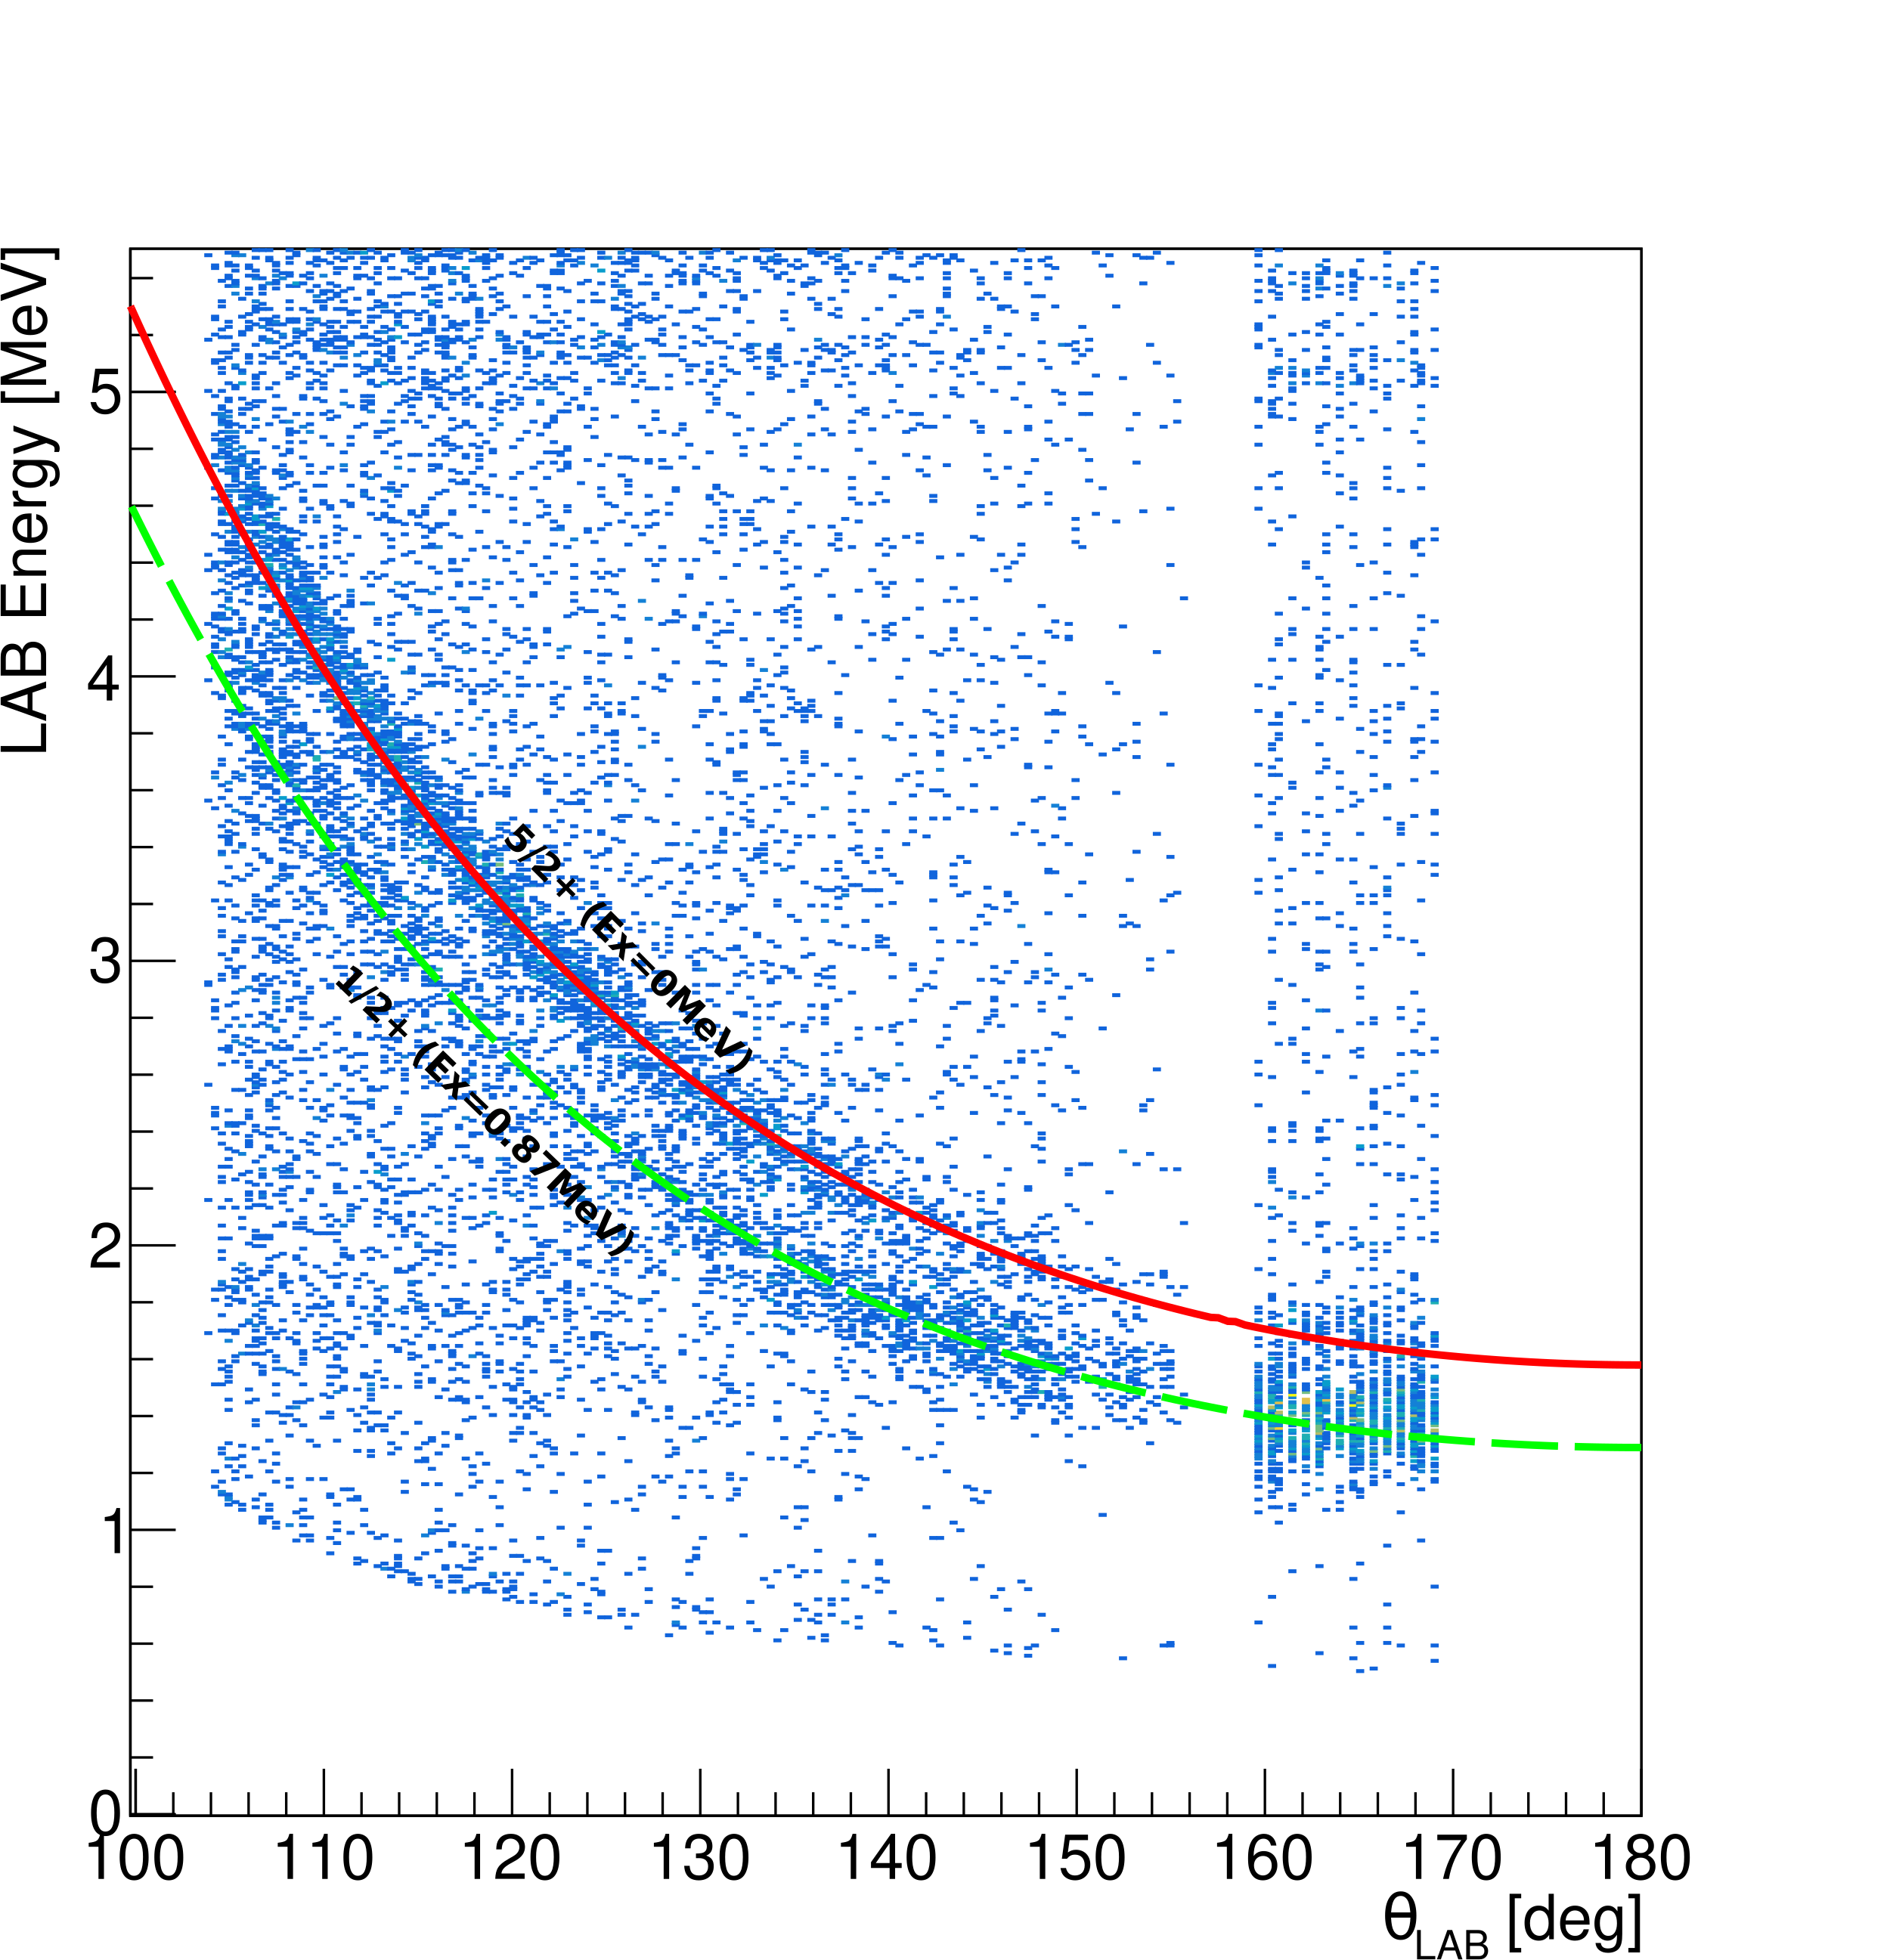
\includegraphics[width=1.2\textwidth]{KineMugast.png}}
		\only<2>{\vspace{0.01\textheight}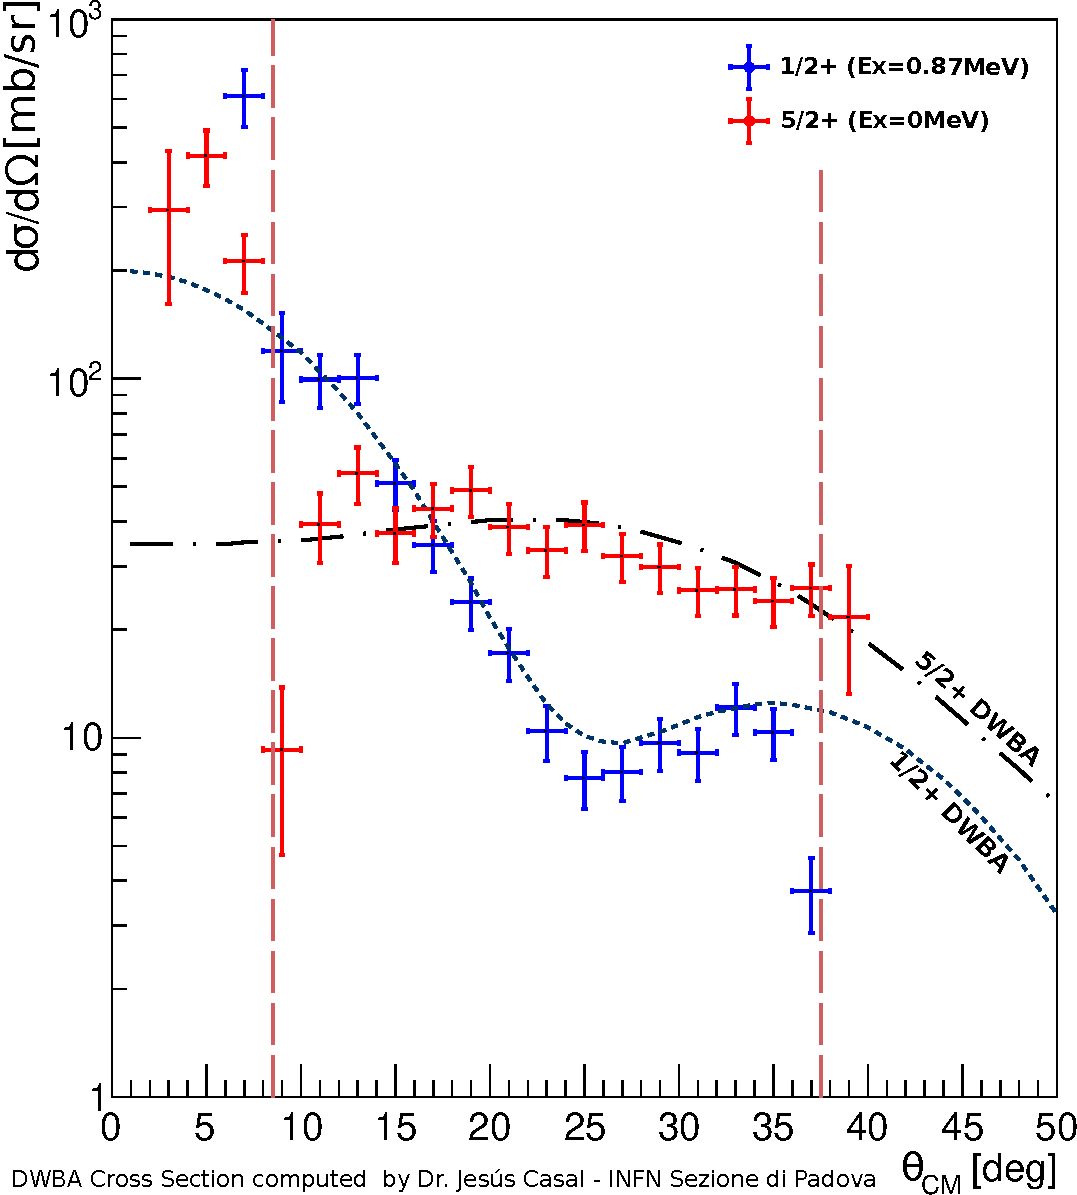
\includegraphics[width=\textwidth]{ADist_jesus}}
		\only<3>{\vspace{0.01\textheight}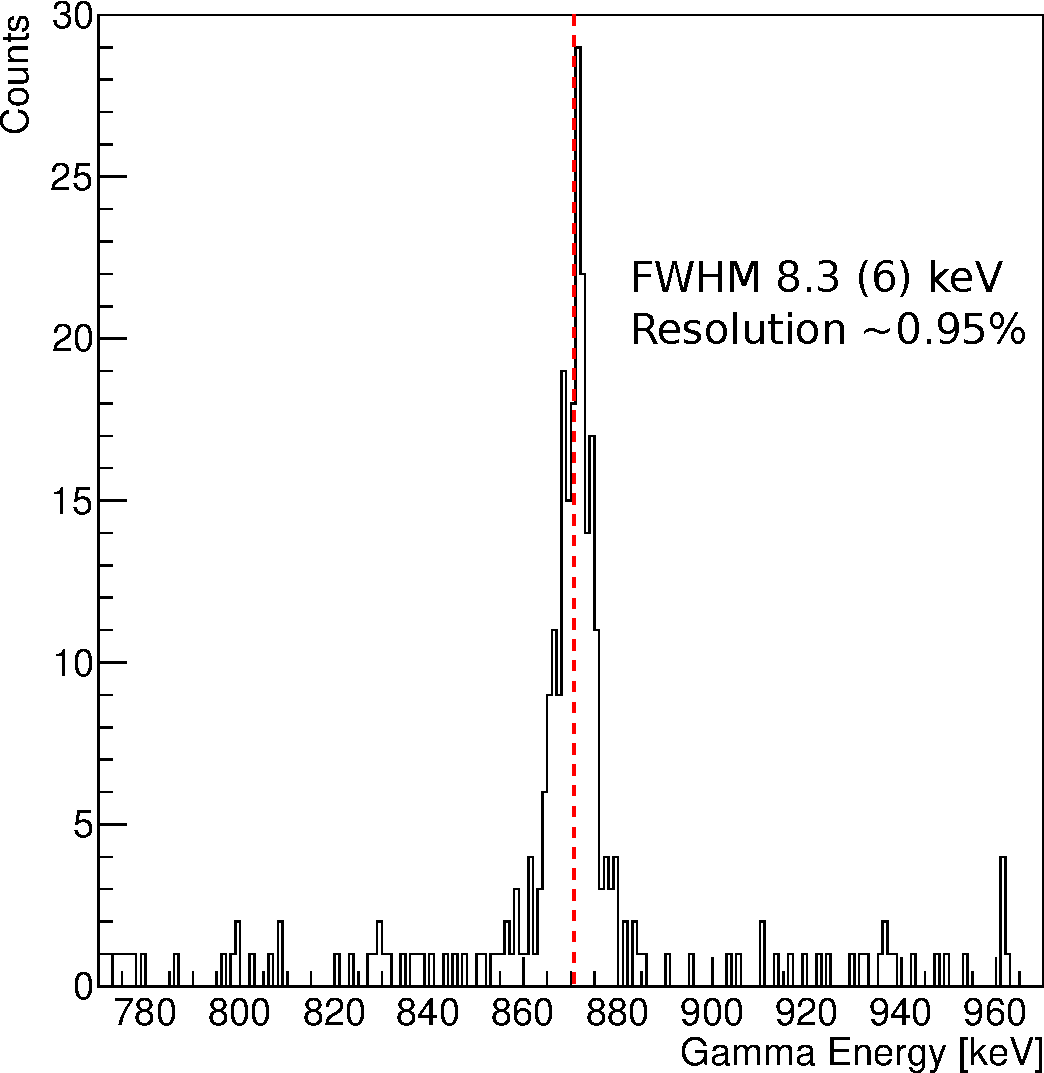
\includegraphics[width=\textwidth]{GammaDP_33shiftResolution}}
		\only<4>{	\vspace{0.1\textheight}
					\begin{align*}
								  \text{\textbf{Add Back}}\ &\rightarrow\ 7.0 \pm 0.5\ \%\\
								  \text{\textbf{Tracking}}\ &\rightarrow\ 6.3 \pm 0.5\ \%
					\end{align*}}
	\end{overlayarea}
\end{column}
\begin{column}{0.6\textwidth}
%\vspace{-0.4\textheight}
\begin{overlayarea}{\textwidth}{\textheight}
\begin{itemize}	
		\item<1-> Kinematic of the outgoing proton and $^{17}$O (5/2+ and 1/2+) final levels selection from excitation energy.
		\item<2-> Angular distribution normalized and fitted to the theoretical differential cross section.
		\item<3-> Coincidence with AGATA and 870~keV peak doppler correction.
		\item<4-> AGATA efficiency estimate
\end{itemize}	
\end{overlayarea}
\end{column}
\end{columns}
\end{frame}